\chapter{Material and Methods} \label{methods}
    This chapter describes the steps taken in this thesis to answer the research question:
        \begin{itemize}
            \item \textit{“As a lightweight vessel do not have the structural capacity to carry all the six echo sounders the \gls{imr} usually deploy, which ones should be prioritized when classifying sandeel in acoustic data?”}
        \end{itemize}
    
    The thesis follows the work of \citeauthor{brautaset2020acoustic}\cite{brautaset2020acoustic}, which was outlined in section \ref{unet_paper_acoustic} and will be referenced throughout this chapter. In summary, this chapter will first look at the data itself and the tools and methods applied to prepare it for the training of machine learning models, with a following description of the experiment. The experiment focuses on training individual U-Net models with different amounts of frequencies and measuring the performance of each.
    
    \section{The Data}
        The data was split into yearly trawl missions, with each consisting of a collection of \textit{.raw} files with corresponding \textit{.work} files. The \textit{.raw} are the uncompressed raw output from the echo sounder. Because they are uncompressed, they do not lose any data, but unfortunately, this also makes them large. The data from 2020 alone which spanned three months took 240 GB of storage space and was accessed by downloading it through Windows Azure (described in appendix \ref{Windows Azure}). The \textit{.work} files are the annotations of the \textit{.raw} files done by operators using a system called the \Gls{lsss}\cite{lsss}. 
    
    \section{Tool: The CRIMAC-Pipeline}
        Based on the work performed by \citeauthor{brautaset2020acoustic}\cite{brautaset2020acoustic}, a pipeline for classifying the acoustic backscatter was created under \gls{imr}s project \gls{crimac}\cite{crimac_pipeline}, and used as a tool throughout this work. The pipeline could be run as one module, to directly get the predictions from the .raw data, or submodules (illustrated in figure \ref{Module_overview_fig}) could be accessed and run separately. All modules were accessed through docker (described in appendix \ref{Docker}), and a majority of their output is the \textit{.zarr} format. This is a format that is compatible with the Python package Zarr (described in appendix \ref{Zarr}), which facilitates NumPy array operations as well as loading of arrays from disk instead of memory, as these can be very large. This section will describe the function of each module used in this thesis.
        
            \subsection{CRIMAC-Pipeline Modules} \label{CRIMAC-pipeline}
              \begin{figure}[H]
                \centering
                \includesvg[inkscapelatex=false,width=0.7\textwidth,keepaspectratio]{figures/module_overveiw.svg}
                \caption[Module overview]{Module overview and output flowchart. The colors of modules and  their output will stay the same for later illustrations. The white modules were unavailable.}
              	\medskip 
                \label{Module_overview_fig}
            \end{figure}

            \begin{description}
              \item[$\bullet$ CRIMAC/Preprocessor:] Preprocesses the \textit{.raw} and \textit{.work} to respectively \textit{.zarr} and \textit{.parquet} files. The output \textit{.zarr} file contained several types of measurements from the trawl missions, like location, \gls{sv}, and temperature. The data extracted for this thesis was the \gls{sv} data and was represented as a multidimensional array of size \textit{frequency} x \textit{ping} x \textit{range} in the  \textit{.zarr} format. \textit{Range} is equivalent to \textit{depth}. The \textit{.parquet} file would act as bitmaps for each class, but the version of this module was unable to produce these at the time of this work. The output \gls{sv} file is illustrated in figure \ref{Module_outputs_illustration_fig}:

              \item[$\bullet$ Pretrained CRIMAC/U-Net:] Using a pretrained U-Net model, it produces a segmentation map of pixel-based probabilities of spatial size \textit{class} x \textit{ping} x \textit{range} where values in each pixel summaries to 1 over all classes. Output classes were \textit{sandeel}, \textit{other} and \textit{background}. The \textit{ignore} class was not included. The pixel maps are illustrated in figure \ref{Module_outputs_illustration_fig}.  By changing the settings, we have the option to train a new U-Net model with the same scheme setup in \citeauthor{brautaset2020acoustic}, but was incompatible with the \textit{.zarr} format and could not be used.
              
              \item[$\bullet$ CRIMAC/Bottom detection:] Identifies the bottom and generates a binary pixel-based map stored as \textit{.zarr}. This is a 2D array of size \textit{ping} x \textit{range}. The output is shown in figure \ref{Module_outputs_illustration_fig}:

            \end{description}
            
        
        \begin{figure}[H]
            \centering
            \includesvg[inkscapelatex=false,width=1\textwidth,keepaspectratio]{figures/output_illustration.svg}
            \caption[Module outputs illustration]{Illustrations of the output from the different modules with one enlarged example from each output. This example is a $500\times500$ crop, while the real data contained millions of pings. The \textit{200kHz} has been transformed to the decibel scale to make the data observable. The color scale is set to be purple at 0, and yellow at 1. White denotes missing values.}
          	\medskip 
            \label{Module_outputs_illustration_fig}
        \end{figure}

    \section{Pseudo Labels} \label{Pseudo label}
        The operator annotations used as labels by \citeauthor{brautaset2020acoustic}\cite{brautaset2020acoustic} was unavailable at the time of writing this thesis, but their method still relied on supervised learning, where each sample has a corresponding label. To solve this, pseudo labels were created by using the aforementioned pretrained CRIMAC/U-Net (section \ref{CRIMAC-pipeline}) module. The data was processed by the module and the segmentation map of pixel-based probabilities for each class was produced. A hard threshold of 0.8 was then applied to the predictions, and all values below was set to 0, and above to 1, hence resulting in a hard mask for each class. This threshold was applied to only include the most certain predictions of the pretrained CRIMAC/U-Net. Below is an example pseudo label:
        
        %These labels will contain some noise, as the model they originate from was not perfect. In the next section, I will explain how I handled this. Due to the weighted cross-entropy loss used during training of the model seen in section \ref{unet_paper_acoustic} the background class were usually very noisy, as this class was lowly weighted. This low weight caused the model to care less about classifying the background correctly, and the two samples in figure \ref{data sample fig} illustrates this. As I was to use the same weighting, this did not pose a large problem but explains noise in later illustrations of the background class, and therefore mentioned.

        \begin{figure}[H]
        \centering
        %\subfloat[Low noise background label.]{
        	\label{subfig:correct}
        	\includesvg[inkscapelatex=false,width=0.9\textwidth,keepaspectratio]{figures/data_sample.svg}
        	%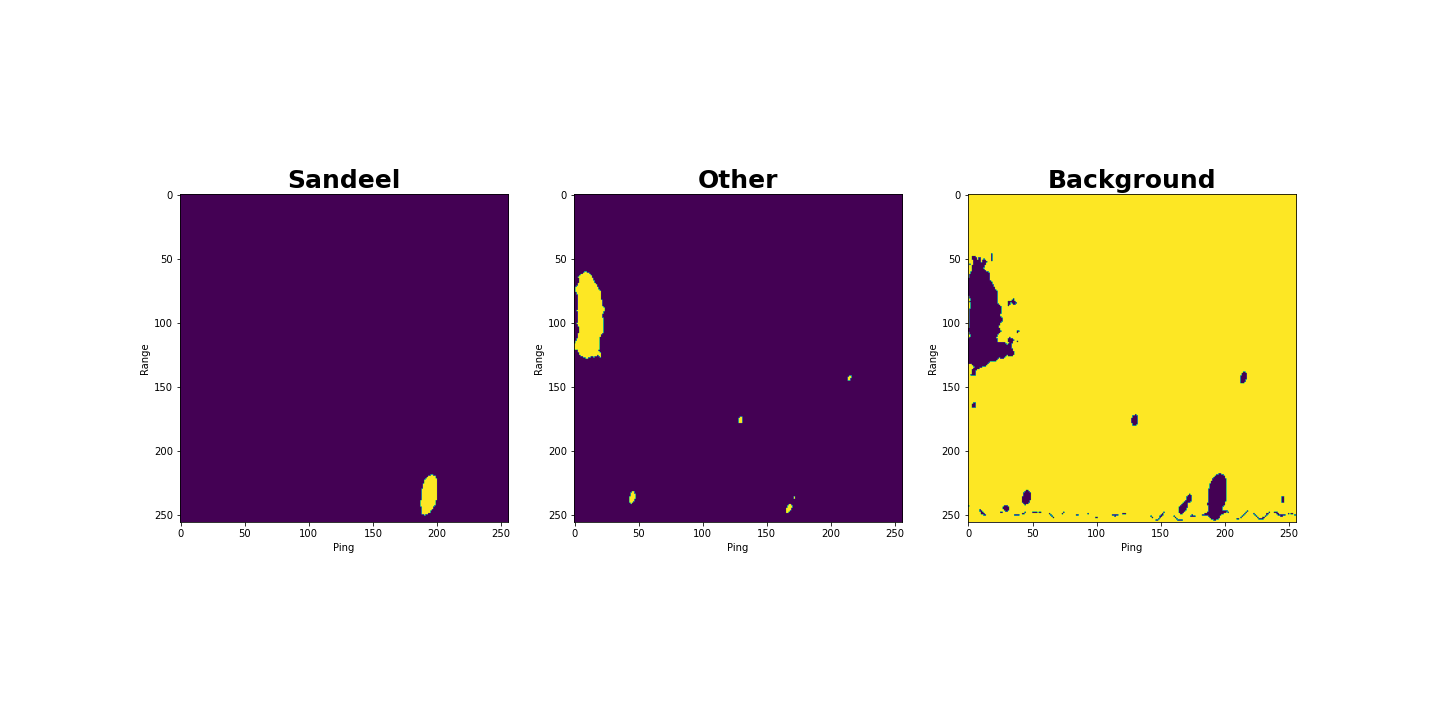
\includegraphics[width=1\textwidth]{figures/data_sample.png} } 
        
        %\subfloat[High noise background label.]{
        	%\label{subfig:notwhitelight}
        	%\includesvg[inkscapelatex=false,width=0.9\textwidth,keepaspectratio]{figures/data_sample_noisy.svg}}
        
        
        \caption[Pseudo label]{An example pseudo label displaying the mask of all three classes present in a 256×256 crop: \textit{Sandeel}, \textit{Other} and \textit{Background}.} %The upper (a) without much noise in the background and the lower (b) containing severe noise.}
        \label{data sample fig}
        
        \end{figure}


        
    \section{Data Preparation}
        This section explains the process of preparing the dataset, which was built to enable a sampling scheme during training equal to the one developed by \citeauthor{brautaset2020acoustic}\cite{brautaset2020acoustic}. In short, the preprocessing consists of creating samples with corresponding pseudo labels from the input data, and storing the samples in a folder structure dependent on the sample's features.
        
        \clearpage
        \begin{figure}[H]
            \centering
            \includesvg[inkscapelatex=false,width=0.75\textwidth,keepaspectratio]{figures/flow_data_gen.svg}
            %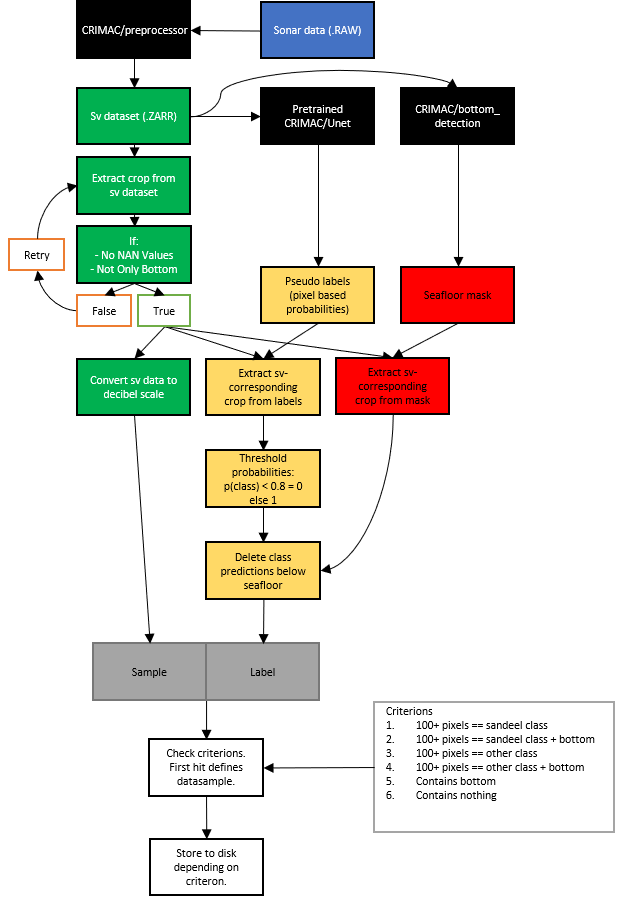
\includegraphics[scale=0.75]{figures/flow_data_gen.png}
            \caption[Data preparation process]{An overview of the data preparation process. CRIMAC pipeline modules (black), data.raw (blue), SV data.zarr (green), pseudo labels.zarr (yellow), bottom.zarr (red), the finished file containing two tensors (gray), storing the file with pickle (white).}
          	\medskip 
            \label{data_generation_flowchart_fig}
        \end{figure}
        
        The entire process is illustrated in figure \ref{data_generation_flowchart_fig} and starts with the utilization of \gls{crimac} preprocessor module as described in \ref{CRIMAC-pipeline}. This takes in the entire \textit{.raw} dataset and outputs the \gls{sv} data in the \textit{.zarr} format. The \gls{sv} dataset was then sent to both the pretrained U-Net and bottom detection modules from the \gls{crimac} pipeline. The pretrained U-Net outputs pseudo labels, and the bottom detection outputs a mask of the seafloor, as arrays equal in spatial size to the \gls{sv} data array.
        
        \begin{figure}[H]
            \centering
            %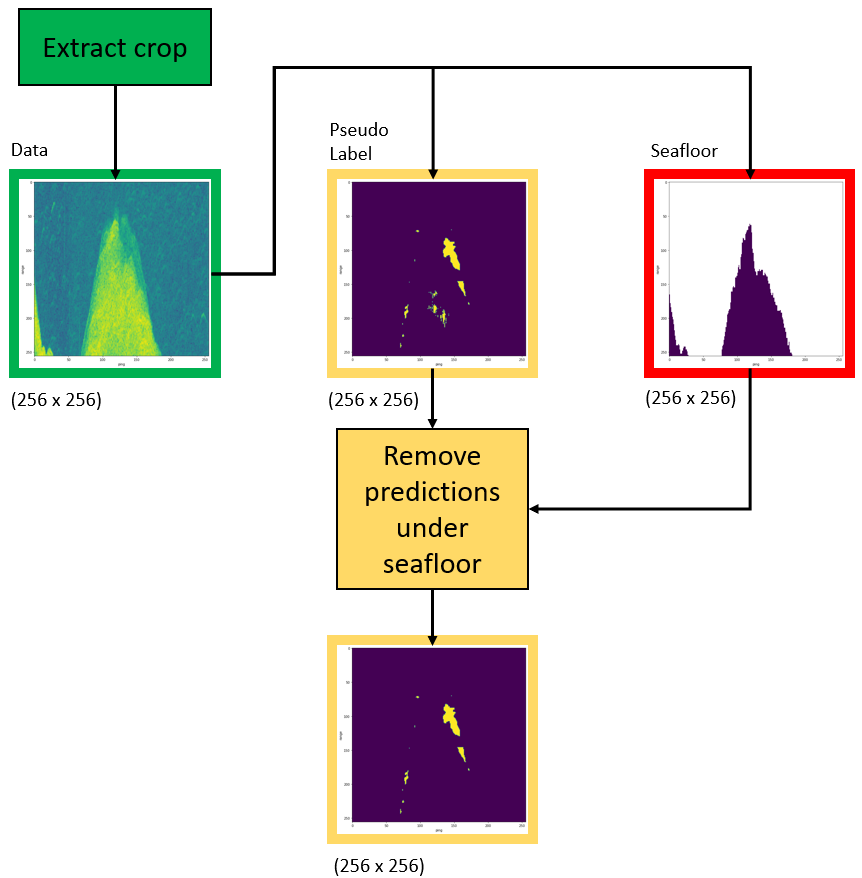
\includegraphics[scale=0.5]{figures/crop_extract_illustration.png}
            \includesvg[inkscapelatex=false,width=0.9\textwidth,keepaspectratio]{figures/data_errors_nans.svg}
            \caption[Missing values and bottom]{Example crop from the 18kHz \gls{sv} data (decibel scale). It illustrates two clear sections of data where the depth (range) is changed, and the gap is filled with missing values (white). The bottom can clearly be observed by the strong line of \gls{sv} values, and there are multiple bottom echoes in certain parts if the crop.}
          	\medskip 
            \label{data_bottom_nans_fig}
        \end{figure}
        
        
        The generated \gls{sv} dataset was then split into non-overlapping crops of size 256x256, ignoring crops of mismatching size at the edges of the array. Each crop was checked for any missing values or the crop being located entirely below the seafloor, and then ignored if any of them were true. This was because missing values can be detrimental to the training process, and crops below the seafloor was excluded as done by \citeauthor{brautaset2020acoustic}\cite{brautaset2020acoustic}. An illustration of the missing data is illustrated in figure \ref{data_bottom_nans_fig}, also showcasing multiple seabfloors that could confuse the model during training. Using the vertical and horizontal coordinates for all the \gls{sv} data crops, a corresponding crop from both the seafloor mask and the pseudo labels were extracted. The two new crops were then used together to remove predictions that appeared under the bottom, thus cleaning and preprocessing the pseudo labels. The steps explained in this paragraph are also visualized in figure \ref{crop_extract_fig}.
        \begin{figure}[H]
            \centering
            %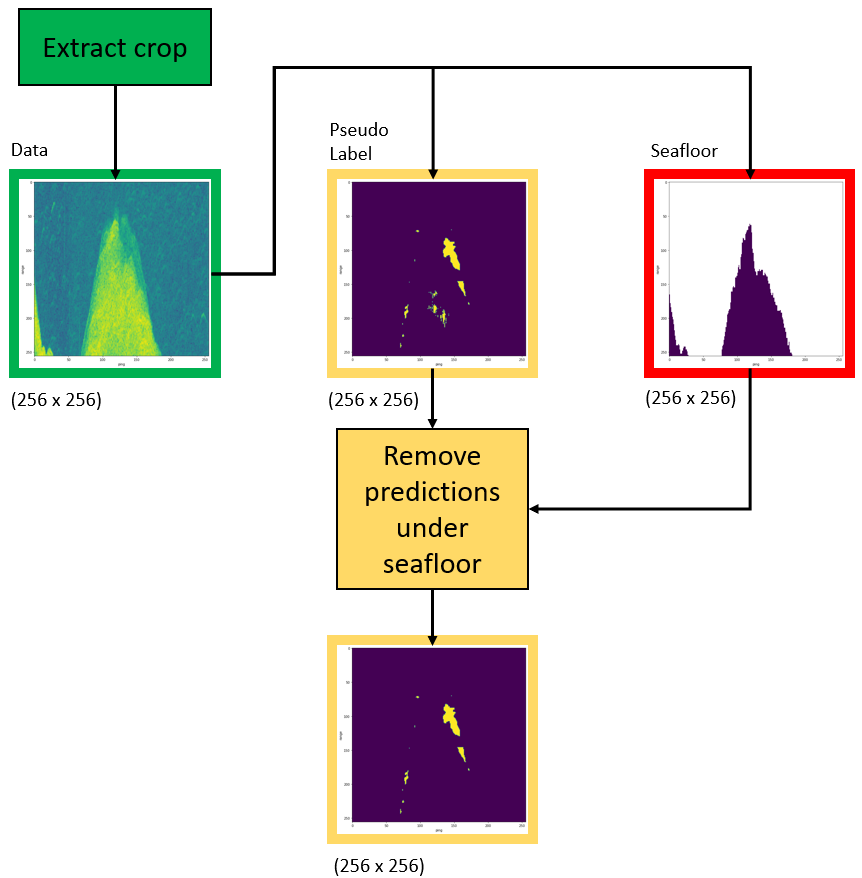
\includegraphics[scale=0.5]{figures/crop_extract_illustration.png}
            \includesvg[inkscapelatex=false,width=0.7\textwidth,keepaspectratio]{figures/crop_extract_illustration.svg}
            \caption[Data, label and bottom crop extraction and interaction]{Example of how the data, pseudo labels and bottom crops would look during data generation. For the pseudo label, purple is values of 0 and yellow values of 1. In the pseudo labels, you can see that some predictions under the seafloor are removed.  Size is shown in the lower-left corner to make it clear that it is a crop of the same size from the same location, but from different arrays.}.
          	\medskip 
            \label{crop_extract_fig}
        \end{figure}
        
        After the crop containing the \gls{sv} data and cleaned pseudo labels were generated, they were both converted to tensors and stored as a single file using pickle\todo{skriv om pickle}. The storage folder of the file would depend on a set of criteria, which are illustrated in figure \ref{data_hierarchy_fig}. The criteria would be checked from top to bottom, and the first triggered would set the destination folder, hence creating a folder structure visualized in figure \ref{data_hierarchy_fig}. This also blocked the same crop from appearing in several folders, potentially causing data leakage between training, validation and test datasets.
        
        
        %\clearpage
        \begin{figure}[H]
            \centering
            %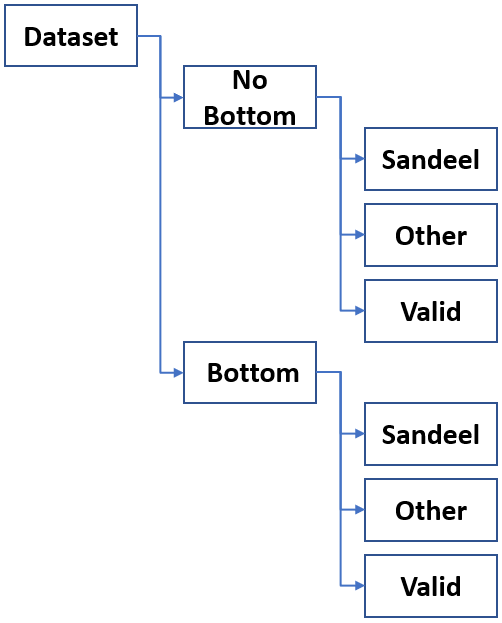
\includegraphics[scale=0.5]{figures/data_hierarki.png}
            \subfloat[List of criteria]{
            \includesvg[inkscapelatex=false,width=0.5\textwidth,keepaspectratio]{figures/criteria.svg}}
            
            \subfloat[Folder structure]{
            \includesvg[inkscapelatex=false,width=0.5\textwidth,keepaspectratio]{figures/folder_structure.svg}}
            


            \caption[Criteria and folder structure]{An overview of the criteria and folder structure. The structure consists of two main branches, one with the bottom present and one without.}
            
            
          	\medskip 
            \label{data_hierarchy_fig}
        \end{figure}
        

        
        The folder structure and criterions were based on the data classes made by \citeauthor{brautaset2020acoustic}\cite{brautaset2020acoustic}. One major difference was that they used the real operator annotations to detect instances of classes in a crop, while we only have the pseudo labels. Since these pseudo labels could contain misclassifications made by the pretrained model, a class abundance measurement was performed. When evaluating the crops against the criteria, if 100 or more pixels in a crop contained either \textit{sandeel} or \textit{other}, it would be set to present in the crop. This would remove crops with low class abundance and where the pretrained model had potentially misclassified single or few pixels. If there were not enough pixels of either class, the crop would be set to contain \textit{background} only. The crop from the \gls{sv} data would be checked against its corresponding crop from the bottom detector output, splitting the data into folders with or without bottom.
        
        The years 2018 and 2019 were processed in the aforementioned way individually, and the final data distribution can be seen in respectively table \ref{data_distribution_2018_table} and \ref{data_distribution_2019_table}.



\begin{longtable}{lllllllll}
\caption[2018 data distribution]{Data distribution for the 2018 dataset.}
\\ \cline{1-4}
\multicolumn{2}{|l|}{\textbf{2018 dataset}} & \multicolumn{1}{l|}{Occurrences} & \multicolumn{1}{l|}{\% of dataset} &  &  &  &  &  \\ \cline{1-4}
\endfirsthead
%
\endhead
%
                     & Sandeel              & 1410                             & 7.3\%                              &  &  &  &  &  \\
No bottom            & Other                & 184                              & 0.95\%                             &  &  &  &  &  \\
                     & Background           & 6519                             & 33.75\%                            &  &  &  &  &  \\ \cline{1-4}
                     & Sandeel              & 1297                             & 6.71\%                             &  &  &  &  &  \\
Bottom               & Other                & 840                              & 4.35\%                             &  &  &  &  &  \\
                     & Background           & 9067                             & 46.94\%                            &  &  &  &  &  \\ \cline{1-4}
\multicolumn{2}{l}{\textbf{Total:}}         & 19317                            & 100\%                              &  &  &  &  &  \\ \cline{1-4}
                     &                      &                                  &                                    &  &  &  &  &  \\
                     &                      &                                  &                                    &  &  &  &  & 
\\ \label{data_distribution_2018_table}
\end{longtable}

% Please add the following required packages to your document preamble:
% \usepackage{longtable}
% Note: It may be necessary to compile the document several times to get a multi-page table to line up properly
\begin{longtable}{lllllllll}
\caption[2019 data distribution]{Data distribution for the 2019 dataset.}
\\ \cline{1-4}
\multicolumn{2}{|l|}{\textbf{2019 dataset}} & \multicolumn{1}{l|}{Occurrences} & \multicolumn{1}{l|}{\% of dataset} &  &  &  &  &  \\ \cline{1-4}
\endfirsthead
%
\endhead
%
                     & Sandeel              & 1308                             & 4.38\%                             &  &  &  &  &  \\
No bottom            & Other                & 1074                             & 3.60\%                             &  &  &  &  &  \\
                     & Background           & 10291                            & 34.45\%                            &  &  &  &  &  \\ \cline{1-4}
                     & Sandeel              & 1652                             & 5.53\%                             &  &  &  &  &  \\
Bottom               & Other                & 2815                             & 9.42\%                             &  &  &  &  &  \\
                     & Background           & 12733                            & 42.62\%                            &  &  &  &  &  \\ \cline{1-4}
\multicolumn{2}{l}{\textbf{Total:}}         & 29873                            & 100\%                              &  &  &  &  &  \\ \cline{1-4}
                     &                      &                                  &                                    &  &  &  &  &  \\
                     &                      &                                  &                                    &  &  &  &  & 
\\ \label{data_distribution_2019_table}
\end{longtable}  

        From the tables above, we observe that as in \citeauthor{brautaset2020acoustic}\cite{brautaset2020acoustic} most of the data will contain no fish, here represented as \textit{background}.

\clearpage
\section{Experiment} \label{Experiment}
    In this section, I will describe how my experiments were performed, and how performance was measured. First by describing the settings, then the experiment itself in detail. In short, the experiment tests different frequency combinations.
    
    \subsection{Experiment Settings} \label{Experiment settings}
        The experiment would use the same U-Net architecture as described in section \ref{unet} with the alteration developed by \citeauthor{brautaset2020acoustic}\cite{brautaset2020acoustic}. The only difference in this work was to adjust the amount of frequency channels in the input layer to test different combinations. This would range from 1 to 6 depending on the number of frequencies in a combination. All machine learning was performed by using PyTorch (described in appendix \ref{Pytorch}).
        
        Data loaded to the model started with first selecting a folder from the folder structure, with a set probability for each. Then a sample would be extracted at random from this folder. This imitates the sampling strategy from \citeauthor{brautaset2020acoustic}\cite{brautaset2020acoustic}, and the probabilities originate from this work.
        
        %\clearpage
        \begin{longtable}{lcl}
            \caption[Data loading scheme]{The sample classes correspond to the folder structure described in figure \ref{data_hierarchy_fig}. Each is given a probability of being the target folder for sample extraction.}
            \\ \hline
             \multicolumn{1}{|l|}{\textbf{Sample class}} &  \multicolumn{1}{l|}{\textbf{Probability}} &  \multicolumn{1}{l|}{\textbf{Details}}                                                         \\ \hline
            \endfirsthead
            %
            \endhead
            
            %
            Sandeel                                     & 5/26                                      & Random crop containing the sandeel class                                                      \\ \hline
            Other                                       & 5/26                                      & Random crop containing the other class                                                        \\ \hline
            Background                                       & 1/26                                      & Random crop containing no fish                                                                \\ \hline
            Sandeel + bottom                          & 5/26                                      & \begin{tabular}[c]{@{}l@{}}Random crop containing the sandeel class\\ and bottom\end{tabular} \\ \hline
            Other + bottom                             & 5/26                                      & \begin{tabular}[c]{@{}l@{}}Random crop containing the other class\\ and bottom\end{tabular}   \\ \hline
            Background + bottom                        & 5/26                                      & \begin{tabular}[c]{@{}l@{}}Random crop containing no fish\\ and bottom\end{tabular}           \\ \hline
            \label{Data_loading_scheme_table}
        \end{longtable}

        The data-augmentations performed was flipping along the vertical axis, and a multiplication applied to values in 5\% of pixels in an input \gls{sv} crop to act as noise. In this context, pixels refer to each \gls{sv} value in the crop. The intention behind the multiplication was to simulate real life noise, and consisted of multiplying the values with a random number in either the range [0,1] or [1, 10], with a 50\% change of each. Then the \gls{sv} crop would be transformed to the decibel scale, by applying $10*\log{(pixel)}$ to all pixels for all frequencies in the \gls{sv} crop, with cutoff values at minimum -75dB and maximum 0dB. As samples from the training data was provided to the model, each data augmentation method had a 50\% chance of occurring. All augmentations and transformations was based on \citeauthor{brautaset2020acoustic}\cite{brautaset2020acoustic}. 

        
        %\clearpage
        \begin{longtable}{lll}

            \caption[Data augmentation summary]{Description of each data augmentation performed.}
            \\\hline
            \multicolumn{2}{|l|}{\textbf{Data augmentation}} & \multicolumn{1}{l|}{\textbf{Details}} \\ \hline
            \endfirsthead
            %
            \endhead
            %
            \textit{Add noise to 5\% of pixels.}      &       & 50\% of occurring upon loading sample \\ \hline
            \textit{Flip along vertical axis}        &       & 50\% of occurring upon loading sample \\ \hline

            \label{data_augmentation_table}
        \end{longtable}
        
        The hyperparameters used during training are summarized in table \ref{hyperparameter_table} and equal those used by \citeauthor{brautaset2020acoustic}\cite{brautaset2020acoustic}.

        \begin{longtable}{lll}
            
            \caption[Experiment hyperparameters]{Settings for all hyperparameters used during the training.}\\
            \\ \hline
            \multicolumn{1}{|l|}{\textbf{Hyperparameters}} & \multicolumn{1}{l|}{\textbf{Value/ Category}} & \multicolumn{1}{l|}{\textbf{Details}}                                                 \\ \hline
            \endfirsthead
            %
            \endhead
            %
            \textit{Loss function:}                         & Weighted Cross-entropy                        & \begin{tabular}[c]{@{}l@{}}Background = 1, \\ Other = 25,\\ Sandeel = 30\end{tabular} \\ \hline
            \textit{Optimizer:}                             & Stochastic gradient descent                   &                                                                                       \\ \hline
            \textit{Learning rate:}                         & 0.01                                          & \begin{tabular}[c]{@{}l@{}}Halved every \\ 1000th batch\end{tabular}                  \\ \hline
            \textit{Momentum:}                              & 0.95                                          &                                                                                       \\ \hline
            \textit{Batch size:}                            & 16                                            &                                                                                       \\ \hline
            \textit{Crop size:}                             & 256×256                                       & \begin{tabular}[c]{@{}l@{}}Include all \\ available channels\end{tabular}             \\ \hline
        \label{hyperparameter_table}
        \end{longtable}

        To evaluate the performance of the models, we utilized the F1 score mentioned in section \ref{f1_score}. We also included the precision and recall, as these provide greater insight to the model's performance.
        
    %\subsection{Experiment: Training on pseudo labels}
    %  This was a preliminary test to establish that training a model on pseudo labels was possible and would achieve acceptable performance. All frequencies would be included, and this would then produce a baseline performance for the later experiments. 
    
    \subsection{Exhaustive Frequency Search}
    
        To find the most impactful frequencies and try to discover hidden synergies between them, a comprehensive test had to be enacted. This experiment would see all combinations of all frequencies being tested. This means to train a U-Net model using only the frequencies in the frequency combination and measure the performance. The experiment would be run ten times, to get enough results to estimate the mean,  reducing variance, and be able to display some statistical data for each combination of frequencies. Each test would have different random state seeds set to enable different data splits, and also model different initialization. The explicit random state also accommodates reproducibility. With 6 frequencies in total, the amount of possible frequency combinations for each of the tests is 63\footnote{Calculated as combinations without repetitions and without order, using formula $\frac{n!}{k!(n-k)!}$, where \textit{n} is elements to chose from and \textit{k} is how many to choose, both values as integers. Summarize for \textit{k} in range 1..6.}.
        
        The dataset for year 2019 in table \ref{data_distribution_2019_table} contained the most data, and this was used for training. 70\% of the 2019 dataset was selected as training dataset, and 30\% as validation dataset. The 2018 dataset was selected as test dataset. The total amount of data given to a model during training was set to 5,000 batches. With a batch size of 16 this corresponds to 80,000 samples, which matches the amount of data given to the model by \citeauthor{brautaset2020acoustic}\cite{brautaset2020acoustic}.
        
        Logging of metrics would occur at different stages during the training process;
            \begin{itemize}
                \item Every minibatch: Calculate running average training loss.
                \item Every minibatch: Logg the running average for both training and validation loss.
                \item Every 500 minibatch: Run model on 100 batches from the validation data, plot one sample output, its label and record running validation loss on each minibatch. Furthermore, calculate F1-score on both training and validation data for every class.
            \end{itemize}
        To accommodate this logging scheme, we split the training process into 50 epochs, with 100 batches in each. This epoch only related to the logging scheme, and not to the data itself. Hence, each epoch is not the entire dataset, but a part of a sequence of data. This is mentioned to not confuse the reader observing the results.
    
        As the logging and random state was equal for all combinations internal in a test, this would create good comparison illustrations of how each combination performed on the same sample. The metrics loss and F1-score would give an indication towards convergence, over-/under-fitting problems and performance. A sanity check would also be performed by observing a prediction of the sandeel class.
        
        After the training of each frequency combination, the network was evaluated on 500 batches from the test data, but without any noise added through augmentation. Finally, the F1-score, precision and recall would be calculated for each class and logged in a \textit{.csv} file. Then the next combination would start the entire process afresh with training.
        
        With the results from the 5 separate experiments, each on all 63 possible combinations, the mean performance values of each frequency combination would be estimated. This would then be used to show these properties:
        \begin{itemize}

            \item Greedy search among the best frequency combinations per number of frequencies possible. For example; The best from all combinations of three frequencies. One greedy search based on each metric; f1-score, precision, and recall.
            \item To observe how unique the performance was for each combination, a plot to illustrate the statistical properties of each will be presented. This will be shown as an error bar, the top of the bar is the max F1-score achieved, and the bottom is the minimum. This presentation was chosen because we judged that too few tests had been run for a proper standard deviation to be calculated.
            \item The performance trend of each frequency. This meant we would, for all frequencies, filter out those sets it was a part of and sort these in increasing order. This would produce a line-plot illustrating what performance scores this frequency contributes to and its overall trend.
        \end{itemize}
    


    